% ============================================================
%  يُترجَم بـ XeLaTeX  (في Overleaf: Menu → Compiler → XeLaTeX)
%  الخط: Amiri (متوفر في Overleaf، أو حمّله من github.com/aliftype/amiri)
% ============================================================
\documentclass[12pt,a4paper]{article}
\usepackage[a4paper,margin=1.7cm,top=2.3cm,bottom=2.9cm,headheight=15pt,footskip=1.5cm]{geometry}
\usepackage{amsmath,amssymb}
\usepackage{icomma}
\usepackage[english,bidi=default,layout=lists]{babel}
\babelprovide[import,main]{arabic}
\babelfont{rm}[Scale=1.08]{Amiri}
\babelfont{sf}[Scale=1.08]{Amiri}
\usepackage[most]{tcolorbox}
\usepackage{tikz}
\usetikzlibrary{arrows.meta,calc,shadings}
\usepackage{array}
\usepackage{colortbl}
\usepackage{fancyhdr}
\usepackage{titlesec}
\usepackage{enumitem}
\usepackage{collcell}
\usepackage{needspace}
\usepackage{etoolbox}
\newcolumntype{C}{>{\collectcell\ar}c<{\endcollectcell}}
\pretocmd{\section}{\Needspace{15\baselineskip}}{}{}
\pretocmd{\subsection}{\Needspace{11\baselineskip}}{}{}

\definecolor{cDef}{HTML}{1F4E9C}
\definecolor{cThm}{HTML}{B3261E}
\definecolor{cRem}{HTML}{2E7D32}
\definecolor{cEx}{HTML}{C76B00}
\definecolor{cMeth}{HTML}{6A1B9A}
\definecolor{cSol}{HTML}{00695C}
\definecolor{cSec}{HTML}{1F3A68}

\titleformat{\section}{\Large\bfseries\color{cSec}}{\thesection.}{0.6em}{}[{\color{cSec!60}\titlerule[1pt]}]
\titleformat{\subsection}{\large\bfseries\color{cThm!85!black}}{\thesubsection.}{0.5em}{}
\titlespacing*{\section}{0pt}{14pt}{8pt}
\titlespacing*{\subsection}{0pt}{10pt}{5pt}
\setlength{\parindent}{0pt}
\setlength{\parskip}{4pt}
\setlist{itemsep=2pt,topsep=3pt}

\newtcolorbox{arbox}[3][]{enhanced,
  colback=#2!5,colframe=#2!80!black,arc=2mm,boxrule=0.8pt,
  left=6pt,right=6pt,top=8pt,bottom=5pt,
  fonttitle=\bfseries,coltitle=white,
  title={\foreignlanguage{arabic}{#3}},
  attach boxed title to top right={xshift=-5mm,yshift=-3mm},
  boxed title style={colback=#2!80!black,arc=1.5mm,boxrule=0pt},
  before upper={\selectlanguage{arabic}},
  before skip=8pt,after skip=8pt,breakable,#1}
\newenvironment{BOX}[2]{\begin{otherlanguage}{english}\begin{arbox}{#1}{#2}}{\end{arbox}\end{otherlanguage}}
\newenvironment{tarif}[1][تعريف]{\begin{BOX}{cDef}{#1}}{\end{BOX}}
\newenvironment{khassia}[1][خاصية]{\begin{BOX}{cThm}{#1}}{\end{BOX}}
\newenvironment{molahada}[1][ملاحظة]{\begin{BOX}{cRem}{#1}}{\end{BOX}}
\newenvironment{mithal}[1][مثال]{\begin{BOX}{cEx}{#1}}{\end{BOX}}
\newenvironment{tariqa}[1][طريقة]{\begin{BOX}{cMeth}{#1}}{\end{BOX}}

\newcounter{exo}
\newenvironment{tamrin}[1]{\stepcounter{exo}\begin{BOX}{cSec}{التمرين \theexo: #1}}{\end{BOX}}
\newenvironment{hal}{\Needspace{12\baselineskip}\begin{otherlanguage}{english}\begin{arbox}[breakable]{cSol}{حل التمرين \theexo}}{\end{arbox}\end{otherlanguage}}

\newenvironment{LTR}{\begin{otherlanguage}{english}}{\end{otherlanguage}}
\newcommand{\ar}[1]{\foreignlanguage{arabic}{#1}}

\renewcommand{\dots}{\mathinner{\ldotp\ldotp\ldotp}}
\renewcommand{\ldots}{\mathinner{\ldotp\ldotp\ldotp}}
\renewcommand{\cdots}{\mathinner{\cdotp\cdotp\cdotp}}
\newcommand{\N}{\mathbb{N}}
\newcommand{\Z}{\mathbb{Z}}
\newcommand{\D}{\mathbb{D}}
\newcommand{\Q}{\mathbb{Q}}
\newcommand{\R}{\mathbb{R}}
\newcommand{\pgcd}{\operatorname{PGCD}}
\newcommand{\ppcm}{\operatorname{PPCM}}

% \NLseg{a}{b}{[}{]} ; \NLright{a}{[} ; \NLleft{b}{]}  (interval on a number line)
\newcommand{\NLseg}[4]{\begin{LTR}\begin{tikzpicture}[baseline=-0.6ex]
 \draw[-{Stealth[length=2mm]},gray!70](0,0)--(3.4,0);
 \draw[line width=2pt,cThm!80!black](0.7,0)--(2.7,0);
 \node[cThm!80!black,font=\LARGE] at (0.7,0){$#3$};
 \node[cThm!80!black,font=\LARGE] at (2.7,0){$#4$};
 \node[below=3pt,font=\footnotesize] at (0.7,0){$#1$};
 \node[below=3pt,font=\footnotesize] at (2.7,0){$#2$};
\end{tikzpicture}\end{LTR}}
\newcommand{\NLright}[2]{\begin{LTR}\begin{tikzpicture}[baseline=-0.6ex]
 \draw[-{Stealth[length=2mm]},gray!70](0,0)--(3.4,0);
 \draw[line width=2pt,cThm!80!black](1.3,0)--(3.3,0);
 \node[cThm!80!black,font=\LARGE] at (1.3,0){$#2$};
 \node[below=3pt,font=\footnotesize] at (1.3,0){$#1$};
\end{tikzpicture}\end{LTR}}
\newcommand{\NLleft}[2]{\begin{LTR}\begin{tikzpicture}[baseline=-0.6ex]
 \draw[-{Stealth[length=2mm]},gray!70](0,0)--(3.4,0);
 \draw[line width=2pt,cThm!80!black](0.05,0)--(2.1,0);
 \node[cThm!80!black,font=\LARGE] at (2.1,0){$#2$};
 \node[below=3pt,font=\footnotesize] at (2.1,0){$#1$};
\end{tikzpicture}\end{LTR}}

% ---------- social-media icons (pure TikZ) ----------
\definecolor{cFB}{HTML}{1877F2}
\definecolor{cTG}{HTML}{229ED9}
\definecolor{cIG1}{HTML}{FEDA75}
\definecolor{cIG2}{HTML}{D62976}
\definecolor{cIG3}{HTML}{4F5BD5}
\newcommand{\fbicon}{\begin{LTR}\begin{tikzpicture}[baseline=-0.75ex,x=1em,y=1em]
 \fill[cFB] (0,0) circle (0.55);
 \node[white,inner sep=0,font=\usefont{TU}{lmss}{bx}{n}\small] at (0.04,-0.02) {f};
\end{tikzpicture}\end{LTR}}
\newcommand{\igicon}{\begin{LTR}
\begin{tikzpicture}[baseline=-0.75ex,x=1em,y=1em]
 \shade[lower left=cIG1,lower right=cIG2,upper left=cIG2,upper right=cIG3,rounded corners=0.28em] (-0.55,-0.55) rectangle (0.55,0.55);
 \draw[white,line width=0.09em,rounded corners=0.18em] (-0.36,-0.36) rectangle (0.36,0.36);
 \draw[white,line width=0.09em] (0,0) circle (0.17);
 \fill[white] (0.22,0.22) circle (0.05);
\end{tikzpicture}\end{LTR}}
\newcommand{\tgicon}{\begin{LTR}
\begin{tikzpicture}[baseline=-0.75ex,x=1em,y=1em]
 \fill[cTG] (0,0) circle (0.55);
 \fill[white] (-0.33,0.0) -- (0.32,0.27) -- (0.2,-0.3) -- (0.0,-0.15) -- (-0.08,-0.28) -- (-0.08,-0.08) -- cycle;
 \fill[cTG!70!black] (-0.08,-0.08) -- (0.25,0.2) -- (0.0,-0.15) -- (-0.08,-0.28) -- cycle;
\end{tikzpicture}\end{LTR}}
% page number: black box, white two-digit number, at the right of the social row
\newcommand{\PageBox}{\begin{LTR}\tikz[baseline=(p.base)]\node[fill=black,text=white,inner sep=2.5pt,minimum width=1.6em,minimum height=1.3em,font=\usefont{TU}{lmss}{bx}{n}\small](p){\ifnum\value{page}<10 0\fi\arabic{page}};\end{LTR}}
% visual left-to-right order: Telegram | Instagram | Facebook | page box
\newcommand{\SocialRow}{\begin{otherlanguage}{english}%
 \ar{\textbf{الأستاذ سوايسية هشام للرياضيات}}\ \tgicon\hfill
 \textbf{prof\_hicham\_math}\ \igicon\hfill
 \ar{\textbf{الأستاذ سوايسية هشام للرياضيات}}\ \fbicon\hspace{2.2em}\PageBox\end{otherlanguage}}

\pagestyle{fancy}
\fancyhf{}
\renewcommand{\headrulewidth}{0.6pt}
\renewcommand{\footrulewidth}{0.4pt}
% \SetHeader{right head: document title}{left head: level -- stream}
\newcommand{\SetHeader}[2]{%
 \fancyhead[C]{\parbox{\textwidth}{\ar{#1\hfill #2}}}%
 \fancyfoot[C]{\parbox{\textwidth}{\small\SocialRow}}}
\usepackage{tkz-tab}
\usepackage{multicol}
% variation / sign table (LTR)
\newenvironment{TAB}{\par\begin{center}\begin{LTR}\begin{tikzpicture}[scale=0.95,every node/.style={font=\small}]}{\end{tikzpicture}\end{LTR}\end{center}}
% grid + axes, clipped: \begin{GR}{xmin}{xmax}{ymin}{ymax}{unit cm}
\newenvironment{GR}[5]{\par\begin{center}\begin{LTR}\begin{tikzpicture}[x=#5cm,y=#5cm,font=\footnotesize]
 \draw[gray!25,very thin] (#1,#3) grid (#2,#4);
 \draw[-{Stealth[length=2mm]}] (#1,0)--(#2+0.3,0) node[below left]{$x$};
 \draw[-{Stealth[length=2mm]}] (0,#3)--(0,#4+0.3) node[below left]{$y$};
 \node[below left] at (0,0){$O$};
 \begin{scope}\clip (#1,#3) rectangle (#2,#4);}
{\end{scope}\end{tikzpicture}\end{LTR}\end{center}}
\newcommand{\Ticks}[2]{\foreach \t in {#1} \node[below,font=\scriptsize] at (\t,0){$\t$}; \foreach \t in {#2} \node[left,font=\scriptsize] at (0,\t){$\t$};}
\newcommand{\bx}[1]{\ensuremath{\colorbox{cDef!12}{$\displaystyle #1$}}}
\newcommand{\TwoCol}[4]{\par\begin{LTR}\noindent\begin{minipage}[t]{#1\textwidth}\selectlanguage{arabic}#2\end{minipage}\hfill\begin{minipage}[t]{#3\textwidth}\selectlanguage{arabic}#4\end{minipage}\end{LTR}\par}
\newcommand{\RL}[4]{\TwoCol{#3}{#4}{#1}{#2}}  % \RL{w1}{right content}{w2}{left content}
\newcommand{\ok}{$\textcolor{cRem}{\checkmark}$}
\newcommand{\limn}{\displaystyle\lim_{n\to+\infty}}
% sub-questions, each on its own line
\newenvironment{sq}{\begin{itemize}[leftmargin=2.4em,itemsep=3pt]}{\end{itemize}}
\newcommand{\qa}{\item[(أ)]}\newcommand{\qb}{\item[(ب)]}\newcommand{\qc}{\item[(جـ)]}\newcommand{\qd}{\item[(د)]}\newcommand{\qe}{\item[(هـ)]}
\newcommand{\pa}{\par\smallskip\textbf{(أ)} }\newcommand{\pb}{\par\smallskip\textbf{(ب)} }\newcommand{\pc}{\par\smallskip\textbf{(جـ)} }\newcommand{\pd}{\par\smallskip\textbf{(د)} }\newcommand{\pe}{\par\smallskip\textbf{(هـ)} }
\newcommand{\QQ}[1]{\par\smallskip\textbf{#1.} }
\newenvironment{tmr}{\stepcounter{exo}\begin{BOX}{cSec}{تمرين محلول \theexo}}{\end{BOX}}
\newcommand{\ABC}[3]{\\[2pt]\begin{tabular}{p{0.28\textwidth}p{0.28\textwidth}p{0.28\textwidth}}(جـ) \ #3 & (ب) \ #2 & (أ) \ #1\end{tabular}}
\pretocmd{\section}{\Needspace{24\baselineskip}}{}{}
\newtcbox{\bxtbox}{on line,colback=cDef!12,colframe=cDef!12,boxrule=0pt,arc=1pt,boxsep=0pt,left=2pt,right=2pt,top=1pt,bottom=1pt}
\newcommand{\bxt}[1]{\foreignlanguage{english}{\bxtbox{\ar{#1}}}}
\usepackage{longtable}
\setlength{\LTpre}{4pt}\setlength{\LTpost}{0pt}
\newcommand{\Phase}[1]{\textbf{#1}}
\newcommand{\Fld}[2]{\textbf{#1:}\ #2}
% رأس المذكرة على نمط النموذج: إطار بعنوان «مذكرة رقم»، معلومات الحصة، ثم إطار الكفاءات
\newcommand{\ModhHead}[9]{%
\begin{LTR}
\begin{tcolorbox}[enhanced,colback=white,colframe=cThm!85!black,arc=4mm,boxrule=1pt,top=14pt,bottom=6pt,left=8pt,right=8pt,
 overlay={\node[fill=cThm!85!black,text=white,rounded corners=3mm,inner xsep=14pt,inner ysep=4pt,font=\large\bfseries] at ([yshift=0pt]frame.north){\ar{مذكرة رقم #1}};},
 before upper={\selectlanguage{arabic}}]
\begin{tabular}{@{}p{0.4\linewidth}p{0.55\linewidth}@{}}
\Fld{المستوى}{#2} & \Fld{الثانوية}{\dotfill}\\[3pt]
\Fld{المادة}{رياضيات} & \Fld{ميدان التعلم}{#3}\\[3pt]
\Fld{المدة}{#5} & \Fld{الوحدة التعلمية}{#4}\\[3pt]
\Fld{الأستاذ}{\dotfill} & \Fld{المحتوى المعرفي}{#6}\\
\end{tabular}
\end{tcolorbox}
\begin{tcolorbox}[enhanced,colback=white,colframe=cThm!85!black,arc=3mm,boxrule=0.8pt,sidebyside,sidebyside align=top,lefthand ratio=0.5,
 segmentation style={dashed,cThm!60},before upper={\selectlanguage{arabic}},before lower={\selectlanguage{arabic}}]
\textbf{الكفاءات المستهدفة:}\par #8
\tcblower
\textbf{الكفاءات القبلية:}\par #7
\end{tcolorbox}
\end{LTR}
\par\smallskip\textbf{الوسائل:} #9\par\smallskip}
\newenvironment{Sayr}{%
\begin{LTR}\renewcommand{\arraystretch}{1.25}
\begin{longtable}{|p{0.17\textwidth}|>{\centering\arraybackslash}p{0.06\textwidth}|p{0.53\textwidth}|>{\centering\arraybackslash}p{0.12\textwidth}|}
\hline\rowcolor{cThm!12}\ar{\textbf{توجيهات وتعاليق}} & \ar{\textbf{المدة}} & \ar{\textbf{سير الحصة}} & \ar{\textbf{مراحل الحصة}}\\\hline\endhead
\hline\endfoot}{\end{longtable}\end{LTR}}
% سطر في الجدول: \Row{مرحلة}{سير}{مدة}{توجيهات}
\newcommand{\Row}[4]{\ar{\small #4} & \ar{#3} & \ar{#2} & \cellcolor{cThm!8}\ar{\Phase{#1}}\\\hline}

\newcommand{\Lab}[2]{\foreignlanguage{english}{\tcbox[on line,colback=#1,colframe=#1,boxrule=0pt,arc=2pt,boxsep=1pt,left=5pt,right=5pt,top=1pt,bottom=1pt]{\ar{\textcolor{white}{\textbf{#2}}}}}}
\newcommand{\Num}[1]{\foreignlanguage{english}{\tikz[baseline=(c.base)]\node[fill=cDef,text=white,inner sep=2pt,font=\footnotesize\bfseries](c){#1};}}
\newcommand{\ck}{\ensuremath{{\color{cRem}\checkmark}}}
\newenvironment{Kad}[1]{\par\smallskip\Lab{#1}}{\par}
\newcommand{\RR}[1]{\ifmmode{\color{cThm}#1}\else$\mbox{\color{cThm}#1}$\fi}
\newcommand{\T}[1]{$\mbox{\color{cDef}\bfseries #1}$}
\SetHeader{\small\bfseries\color{cSec}مذكرات محور: النهايات ودراسة الدوال}{\small\color{cSec}السنة الثالثة ثانوي -- تسيير واقتصاد}
\begin{document}
\begin{LTR}
\begin{tcolorbox}[enhanced,colback=cThm!85!black,colframe=cThm!85!black,arc=3mm,halign=center,boxrule=0pt,top=12pt,bottom=12pt,before upper={\selectlanguage{arabic}}]
{\color{white}\fontsize{24}{30}\selectfont\bfseries مذكرات محور: النهايات ودراسة الدوال}\\[8pt]
{\color{white}\large السنة الثالثة ثانوي -- تسيير واقتصاد}\\[4pt]
{\color{white}\large 7 مذكرات (14 ساعة) -- السنة الدراسية 2026-2027}
\end{tcolorbox}
\end{LTR}
\begin{BOX}{cThm}{يتضمن هذا العمل}
\begin{enumerate}[label=\textbf{مذكرة \arabic{enumi}:},leftmargin=6em,start=15]
\item النهايات المرجعية والعمليات على النهايات.
\item نهاية كثير حدود أو دالة ناطقة عند $\pm\infty$ ، إزالة عدم التعيين.
\item نهاية دالة مركبة ، النهاية بالمقارنة.
\item المستقيمات المقاربة الموازية للمحورين ، الوضع النسبي.
\item المستقيم المقارب المائل ، الوضع النسبي.
\item حل مسائل: دراسة دالة ناطقة.
\item حل مسائل: دراسة دالة الكلفة المتوسطة.
\end{enumerate}
الحلول مفصّلة: المعطيات بالأسود ، \T{العناوين} و\RR{النتائج} بلون مختلف ، وكل سؤال في سطر.
\end{BOX}
\newpage
\ModhHead{15}{3 ت ا}{تحليل}{النهايات ودراسة الدوال}{02 سا}{النهايات المرجعية والعمليات على النهايات}%
{\begin{itemize}\item النهايات (2 ت ا) ، الدوال المرجعية.\end{itemize}}%
{\begin{itemize}\item حساب نهاية مجموع أو جداء أو حاصل قسمة دالتين.\item التعرف على حالات عدم التعيين.\end{itemize}}%
{المنهاج ، الكتاب المدرسي ، الآلة الحاسبة البيانية.}
\begin{Sayr}
\Row{مرحلة الانطلاق}{%
\textbf{التهيئة النفسية:} إذا كان $f(x)\to+\infty$ و $g(x)\to+\infty$ ، فإلى أين يؤول $f(x)-g(x)$ ؟}{10 د}{تقويم تشخيصي.}
\Row{التشخيص والاكتشاف}{%
\Lab{cEx}{نشاط 01}\par\textbf{(1)} احسب $\lim\limits_{x\to +\infty}(x^2-x)$.\par\textbf{(2)} احسب $\lim\limits_{x\to +\infty}(x-x^2)$.\par\textbf{(3)} احسب $\lim\limits_{x\to +\infty}\big((x+1)-x\big)$. ماذا تستنتج؟}{35 د}{أمثلة مضادة.}
\Row{}{%
\Lab{cDef}{مناقشة النشاط}\par\textbf{(1)} $x^2-x=x(x-1)$: جداء $+\infty\times(+\infty)$ ، إذن $\RR{\lim\limits_{x\to +\infty}(x^2-x)=+\infty}$.\par\textbf{(2)} $x-x^2=x(1-x)$: جداء $+\infty\times(-\infty)$ ، إذن $\RR{\lim\limits_{x\to +\infty}(x-x^2)=-\infty}$.\par\textbf{(3)} $(x+1)-x=1$ ، إذن النهاية $\RR{1}$. الشكل «$+\infty-\infty$» أعطى ثلاث نتائج مختلفة: إنه \RR{حالة عدم تعيين}.}{}{}
\Row{بناء المعارف}{%
\Lab{cThm}{نهايات مرجعية}\par\textbf{(1)} $\lim\limits_{x\to +\infty}x^n=+\infty$ ؛ $\lim\limits_{x\to -\infty}x^n=+\infty$ إذا كان $n$ زوجياً ، و $-\infty$ إذا كان فردياً.\par\textbf{(2)} $\lim\limits_{x\to \pm\infty}\dfrac1{x^n}=0$ ؛ $\lim\limits_{x\to +\infty}\sqrt x=+\infty$.\par\textbf{(3)} $\lim\limits_{x\to 0^{+}}\dfrac1x=+\infty$ ؛ $\lim\limits_{x\to 0^{-}}\dfrac1x=-\infty$.}{50 د}{الجداول في الكراس.}
\Row{}{%
\Lab{cThm}{نهاية المجموع}\par\smallskip\begin{LTR}\centering {\footnotesize\renewcommand{\arraystretch}{1.45}\setlength{\tabcolsep}{2pt}\begin{tabular}{|>{\centering\arraybackslash}p{0.260\linewidth}|>{\centering\arraybackslash}p{0.120\linewidth}|>{\centering\arraybackslash}p{0.120\linewidth}|>{\centering\arraybackslash}p{0.120\linewidth}|>{\centering\arraybackslash}p{0.120\linewidth}|>{\centering\arraybackslash}p{0.120\linewidth}|}\hline\rowcolor{cSec!12}$\lim f$ & $l$ & $l$ & $+\infty$ & $-\infty$ & $+\infty$\\\hline$\lim g$ & $l^{\prime}$ & $\pm\infty$ & $+\infty$ & $-\infty$ & $-\infty$\\\hline$\lim(f+g)$ & $l+l^{\prime}$ & $\pm\infty$ & $+\infty$ & $-\infty$ & \ar{ح ع ت}\\\hline\end{tabular}}\end{LTR}\par }{}{}
\Row{}{%
\Lab{cThm}{نهاية الجداء}\ (إشارة النتيجة بقاعدة الإشارات)\par\smallskip\begin{LTR}\centering {\footnotesize\renewcommand{\arraystretch}{1.45}\setlength{\tabcolsep}{2pt}\begin{tabular}{|>{\centering\arraybackslash}p{0.260\linewidth}|>{\centering\arraybackslash}p{0.150\linewidth}|>{\centering\arraybackslash}p{0.150\linewidth}|>{\centering\arraybackslash}p{0.150\linewidth}|>{\centering\arraybackslash}p{0.150\linewidth}|}\hline\rowcolor{cSec!12}$\lim f$ & $l$ & $l\neq0$ & $\infty$ & $0$\\\hline$\lim g$ & $l^{\prime}$ & $\infty$ & $\infty$ & $\infty$\\\hline$\lim(f\times g)$ & $l\,l^{\prime}$ & $\infty$ & $\infty$ & \ar{ح ع ت}\\\hline\end{tabular}}\end{LTR}\par }{}{}
\Row{}{%
\Lab{cThm}{نهاية حاصل القسمة}\par\smallskip\begin{LTR}\centering {\footnotesize\renewcommand{\arraystretch}{1.45}\setlength{\tabcolsep}{2pt}\begin{tabular}{|>{\centering\arraybackslash}p{0.260\linewidth}|>{\centering\arraybackslash}p{0.100\linewidth}|>{\centering\arraybackslash}p{0.100\linewidth}|>{\centering\arraybackslash}p{0.100\linewidth}|>{\centering\arraybackslash}p{0.100\linewidth}|>{\centering\arraybackslash}p{0.100\linewidth}|>{\centering\arraybackslash}p{0.100\linewidth}|}\hline\rowcolor{cSec!12}$\lim f$ & $l$ & $l$ & $l\neq0$ & $\infty$ & $\infty$ & $0$\\\hline$\lim g$ & $l^{\prime}\neq0$ & $\infty$ & $0$ & $l^{\prime}$ & $\infty$ & $0$\\\hline$\lim\dfrac fg$ & $\dfrac l{l^{\prime}}$ & $0$ & $\infty$ & $\infty$ & \ar{ح ع ت} & \ar{ح ع ت}\\\hline\end{tabular}}\end{LTR}\par }{}{}
\Row{}{%
\Lab{cRem}{ملاحظات}\ حالات عدم التعيين الأربع: $\infty-\infty$ ، $0\times\infty$ ، $\dfrac\infty\infty$ ، $\dfrac00$.}{}{}
\Row{التقويم}{%
\Lab{cMeth}{تمرين تطبيقي}\par\textbf{(1)} احسب $\lim\limits_{x\to +\infty}(x+1)\sqrt x$.\par\textbf{(2)} احسب $\lim\limits_{x\to -\infty}\dfrac1{x^2+1}$.\par\textbf{(3)} احسب $\lim\limits_{x\to 2^{+}}\dfrac{x+1}{x-2}$.}{25 د}{تقويم فردي.}
\Row{}{%
\Lab{cEx}{حل التمرين التطبيقي}\par\textbf{(1)} $x+1\to+\infty$ و $\sqrt x\to+\infty$: الجداء $\RR{+\infty}$.\par\textbf{(2)} $x^2+1\to+\infty$ ، إذن مقلوبه يؤول إلى $\RR{0}$.\par\textbf{(3)} البسط يؤول إلى $3$ ، والمقام $x-2\to0^{+}$ (لأن $x>2$): $\dfrac3{0^{+}}=\RR{+\infty}$.\par\textbf{واجب منزلي:} تمارين من باب النهايات.\par\smallskip\textbf{ملاحظات حول سير الحصة:} \dotfill}{}{}
\end{Sayr}
\newpage
\ModhHead{16}{3 ت ا}{تحليل}{النهايات ودراسة الدوال}{02 سا}{نهاية دالة كثير حدود أو دالة ناطقة عند $\pm\infty$ ، إزالة عدم التعيين}%
{\begin{itemize}\item العمليات على النهايات ، التحليل.\end{itemize}}%
{\begin{itemize}\item تطبيق قاعدة الحدود الأعلى درجة عند $\pm\infty$.\item إزالة حالة $\frac00$ بالتحليل والاختزال.\end{itemize}}%
{المنهاج ، الكتاب المدرسي ، الآلة الحاسبة البيانية.}
\begin{Sayr}
\Row{مرحلة الانطلاق}{%
\textbf{التهيئة النفسية:} $\lim\limits_{x\to +\infty}(x^2-5x)$: لماذا لا نستطيع الحساب مباشرة؟}{10 د}{سؤال تشخيصي.}
\Row{التشخيص والاكتشاف}{%
\Lab{cEx}{نشاط 02}\par\textbf{(1)} بيّن أن $x^2-5x=x^2\left(1-\dfrac5x\right)$ واستنتج $\lim\limits_{x\to +\infty}(x^2-5x)$.\par\textbf{(2)} بيّن أن $\dfrac{2x^2+x}{x^2-3}=\dfrac{2+\frac1x}{1-\frac3{x^2}}$ واستنتج نهايتها عند $+\infty$.}{35 د}{التحليل بالعامل المشترك.}
\Row{}{%
\Lab{cDef}{مناقشة النشاط}\par\textbf{(1)} بالنشر: $x^2\left(1-\dfrac5x\right)=x^2-5x$. و $1-\dfrac5x\to1$ ، إذن الجداء $+\infty\times1=\RR{+\infty}$.\par\textbf{(2)} نقسم البسط والمقام على $x^2$: $\dfrac{2x^2+x}{x^2-3}=\dfrac{2+\frac1x}{1-\frac3{x^2}}\to\dfrac{2+0}{1-0}=\RR{2}$.}{}{}
\Row{}{%
\Lab{cRem}{ملاحظات}\ الحد الأعلى درجة هو الذي «يتحكم» في النهاية عند المالانهاية.}{}{}
\Row{بناء المعارف}{%
\Lab{cThm}{عند $\pm\infty$}\par\textbf{(1)} نهاية كثير حدود هي \RR{نهاية حده الأعلى درجة}.\par\textbf{(2)} نهاية دالة ناطقة هي \RR{نهاية حاصل قسمة الحدين الأعليين درجة}.}{50 د}{نقارن الطرق.}
\Row{}{%
\Lab{cEx}{مثال 1}\ $\lim\limits_{x\to +\infty}(-2x^3+x-5)=\lim\limits_{x\to +\infty}(-2x^3)=\RR{-\infty}$.}{}{}
\Row{}{%
\Lab{cEx}{مثال 2}\par\textbf{(1)} $\lim\limits_{x\to -\infty}\dfrac{x^2+1}{x-2}=\lim\limits_{x\to -\infty}\dfrac{x^2}x=\lim\limits_{x\to -\infty}x=\RR{-\infty}$.\par\textbf{(2)} $\lim\limits_{x\to +\infty}\dfrac{x+1}{x^2+3}=\lim\limits_{x\to +\infty}\dfrac x{x^2}=\lim\limits_{x\to +\infty}\dfrac1x=\RR{0}$.}{}{}
\Row{}{%
\Lab{cMeth}{حالة $\frac00$ عند عدد}\ نحلل البسط والمقام ونختزل:\par $\lim\limits_{x\to 2}\dfrac{x^2-5x+6}{x-2}=\lim\limits_{x\to 2}\dfrac{(x-2)(x-3)}{x-2}=\lim\limits_{x\to 2}(x-3)=\RR{-1}$.}{}{}
\Row{}{%
\Lab{cThm!80!black}{حذار}\ قاعدة الحدود الأعلى درجة صالحة عند $\pm\infty$ فقط.}{}{}
\Row{التقويم}{%
\Lab{cMeth}{تمرين تطبيقي}\par\textbf{(1)} احسب $\lim\limits_{x\to -\infty}\dfrac{3x^2-x}{1-2x^2}$.\par\textbf{(2)} احسب $\lim\limits_{x\to +\infty}\dfrac{x^3-x}{2x^3+1}$.\par\textbf{(3)} احسب $\lim\limits_{x\to 3}\dfrac{x^2-9}{x-3}$.}{25 د}{تقويم فردي.}
\Row{}{%
\Lab{cEx}{حل التمرين التطبيقي}\par\textbf{(1)} $\lim\limits_{x\to -\infty}\dfrac{3x^2}{-2x^2}=\RR{-\dfrac32}$.\par\textbf{(2)} $\lim\limits_{x\to +\infty}\dfrac{x^3}{2x^3}=\RR{\dfrac12}$.\par\textbf{(3)} حالة $\frac00$: $\dfrac{(x-3)(x+3)}{x-3}=x+3$ ، والنهاية $3+3=\RR{6}$.\par\textbf{واجب منزلي:} تمارين من باب النهايات.\par\smallskip\textbf{ملاحظات حول سير الحصة:} \dotfill}{}{}
\end{Sayr}
\newpage
\ModhHead{17}{3 ت ا}{تحليل}{النهايات ودراسة الدوال}{02 سا}{نهاية دالة مركبة ، النهاية بالمقارنة}%
{\begin{itemize}\item مركب دالتين ، العمليات على النهايات.\end{itemize}}%
{\begin{itemize}\item حساب نهاية دالة مركبة.\item تعيين نهاية بالمقارنة وتفسيرها بيانياً.\end{itemize}}%
{المنهاج ، الكتاب المدرسي ، الآلة الحاسبة البيانية.}
\begin{Sayr}
\Row{مرحلة الانطلاق}{%
\textbf{التهيئة النفسية:} إلى أين يؤول $\sqrt{\dfrac{4x+1}{x+2}}$ لما يكبر $x$ كثيراً؟}{10 د}{سؤال.}
\Row{التشخيص والاكتشاف}{%
\Lab{cEx}{نشاط 03}\par\textbf{(1)} احسب $\lim\limits_{x\to +\infty}\dfrac{4x+1}{x+2}$.\par\textbf{(2)} استنتج $\lim\limits_{x\to +\infty}\sqrt{\dfrac{4x+1}{x+2}}$.}{35 د}{المخطط بالأسهم.}
\Row{}{%
\Lab{cDef}{مناقشة النشاط}\par\textbf{(1)} $\lim\limits_{x\to +\infty}\dfrac{4x}{x}=\RR{4}$.\par\textbf{(2)} نضع $X=\dfrac{4x+1}{x+2}$: $X\to4$ و $\lim\limits_{X\to4}\sqrt X=2$ ، إذن النهاية $\RR{2}$.}{}{}
\Row{بناء المعارف}{%
\Lab{cThm}{نهاية دالة مركبة (تُقبل)}\ إذا كان $\lim\limits_{x\to a}u(x)=b$ و $\lim\limits_{X\to b}g(X)=c$ فإن $\RR{\lim\limits_{x\to a}g\big(u(x)\big)=c}$.}{50 د}{رسم بالحاسبة البيانية.}
\Row{}{%
\Lab{cEx}{مثال}\par\textbf{(1)} $\lim\limits_{x\to -\infty}\left(\dfrac{2x-1}{x+3}\right)^2$: $\dfrac{2x-1}{x+3}\to2$ ، إذن النهاية $2^2=\RR{4}$.\par\textbf{(2)} $\lim\limits_{x\to +\infty}\sqrt{x^2+1}$: $x^2+1\to+\infty$ ، إذن النهاية $\RR{+\infty}$.}{}{}
\Row{}{%
\Lab{cThm}{النهاية بالمقارنة (تُقبل)}\par\textbf{(1)} إذا كان $f(x)\geqslant g(x)$ بجوار $+\infty$ و $g(x)\to+\infty$ فإن $\RR{f(x)\to+\infty}$.\par\textbf{(2)} إذا كان $f(x)\leqslant g(x)$ و $g(x)\to-\infty$ فإن $\RR{f(x)\to-\infty}$.\par\textbf{(3)} إذا كان $g(x)\leqslant f(x)\leqslant h(x)$ و $\lim g=\lim h=l$ فإن $\RR{\lim f=l}$.}{}{}
\Row{}{%
\Lab{cRem}{ملاحظات}\ بيانياً: منحنى $f$ محصور بين منحنيين يقتربان من نفس المستقيم $y=l$.}{}{}
\Row{التقويم}{%
\Lab{cMeth}{تمرين تطبيقي}\par\textbf{(1)} احسب $\lim\limits_{x\to +\infty}\dfrac1{(1-2x)^2}$.\par\textbf{(2)} دالة $f$ تحقق من أجل $x>0$: $2-\dfrac1x\leqslant f(x)\leqslant2+\dfrac1x$. احسب $\lim\limits_{x\to +\infty}f(x)$ وفسّر بيانياً.}{25 د}{تقويم فردي.}
\Row{}{%
\Lab{cEx}{حل التمرين التطبيقي}\par\textbf{(1)} $(1-2x)^2\to+\infty$ ، إذن مقلوبه يؤول إلى $\RR{0}$.\par\textbf{(2)} $2-\dfrac1x\to2$ و $2+\dfrac1x\to2$ ، إذن حسب النهاية بالمقارنة $\RR{\lim\limits_{x\to +\infty}f(x)=2}$ ، والمستقيم $y=2$ مقارب أفقي لـ $(C_f)$.\par\textbf{واجب منزلي:} تمارين من باب النهايات.\par\smallskip\textbf{ملاحظات حول سير الحصة:} \dotfill}{}{}
\end{Sayr}
\newpage
\ModhHead{18}{3 ت ا}{تحليل}{النهايات ودراسة الدوال}{02 سا}{المستقيمات المقاربة الموازية لمحوري الإحداثيات ، الوضع النسبي}%
{\begin{itemize}\item النهايات عند $\pm\infty$ وعند عدد.\end{itemize}}%
{\begin{itemize}\item تعيين المستقيمات المقاربة الموازية للمحورين.\item دراسة الوضع النسبي لمنحنٍ ومستقيم مقارب.\end{itemize}}%
{المنهاج ، الكتاب المدرسي ، الآلة الحاسبة البيانية.}
\begin{Sayr}
\Row{مرحلة الانطلاق}{%
\textbf{التهيئة النفسية:} كلفة متوسطة $C_M(q)=5+\dfrac{100}q$: ماذا يحدث لها لما تكبر الكمية؟}{10 د}{وضعية اقتصادية.}
\Row{التشخيص والاكتشاف}{%
\Lab{cEx}{نشاط 04}\par\textbf{(1)} احسب $C_M(10)$ ، $C_M(100)$ ، $C_M(1000)$.\par\textbf{(2)} احسب $\lim\limits_{q\to+\infty}C_M(q)$.\par\textbf{(3)} ادرس إشارة $C_M(q)-5$.}{35 د}{جداول قيم.}
\Row{}{%
\Lab{cDef}{مناقشة النشاط}\par\textbf{(1)} $C_M(10)=5+10=\RR{15}$ ؛ $C_M(100)=5+1=\RR{6}$ ؛ $C_M(1000)=\RR{5{,}1}$.\par\textbf{(2)} $\dfrac{100}q\to0$ ، إذن $\RR{\lim C_M(q)=5}$: المستقيم $y=5$ مقارب أفقي.\par\textbf{(3)} $C_M(q)-5=\dfrac{100}q>0$: المنحنى \RR{فوق} المستقيم $y=5$.}{}{}
\Row{بناء المعارف}{%
\Lab{cDef}{تعريف}\par\textbf{(1)} إذا كان $\lim\limits_{x\to \pm\infty}f(x)=l$ فإن المستقيم $\RR{y=l}$ \textbf{مقارب أفقي} لـ $(C_f)$.\par\textbf{(2)} إذا كان $\lim\limits_{x\to a}f(x)=\pm\infty$ فإن المستقيم $\RR{x=a}$ \textbf{مقارب عمودي} لـ $(C_f)$.}{50 د}{نرسم المقارب بالمتقطع.}
\Row{}{%
\Lab{cMeth}{الوضع النسبي}\ ندرس إشارة $f(x)-l$: موجبة يعني $(C_f)$ فوق $y=l$ ، سالبة يعني تحته.}{}{}
\Row{}{%
\Lab{cEx}{مثال}\ $f(x)=\dfrac{3x-1}{x+2}$ على $\mathbb R-\{-2\}$:\par\textbf{(1)} $\lim\limits_{x\to \pm\infty}f(x)=\lim\limits_{x\to \pm\infty}\dfrac{3x}x=3$: \RR{$y=3$ مقارب أفقي}.\par\textbf{(2)} البسط يؤول إلى $-7$ لما $x\to-2$ ؛ $\lim\limits_{x\to -2^{+}}f(x)=\dfrac{-7}{0^{+}}=-\infty$ و $\lim\limits_{x\to -2^{-}}f(x)=\dfrac{-7}{0^{-}}=+\infty$: \RR{$x=-2$ مقارب عمودي}.\par\textbf{(3)} $f(x)-3=\dfrac{3x-1-3x-6}{x+2}=\dfrac{-7}{x+2}$:\par\smallskip\begin{LTR}\centering {\renewcommand{\arraystretch}{1.6}\setlength{\tabcolsep}{1pt}\begin{tabular}{|>{\centering\arraybackslash}p{0.240\linewidth}|>{\centering\arraybackslash}p{0.144\linewidth}>{\centering\arraybackslash}p{0.144\linewidth}>{\centering\arraybackslash}p{0.144\linewidth}>{\centering\arraybackslash}p{0.144\linewidth}>{\centering\arraybackslash}p{0.144\linewidth}|}\hline\rowcolor{cSec!12}$x$ & $-\infty$ &  & $-2$ &  & $+\infty$\\\hline $f(x)-3$ &  & $+$ & $||$ & $-$ & \\\hline \ar{الوضع النسبي} &  & \ar{$(C_f)$ فوق} & $||$ & \ar{$(C_f)$ تحت} & \\\hline \end{tabular}}\end{LTR}\par }{}{}
\Row{}{%
\Lab{cThm!80!black}{حذار}\ نحدد إشارة المقام $0^{+}$ أو $0^{-}$ قبل الاستنتاج.}{}{}
\Row{التقويم}{%
\Lab{cMeth}{تمرين تطبيقي}\par $g(x)=1+\dfrac2{x-3}$.\par\textbf{(1)} عيّن المستقيمات المقاربة لـ $(C_g)$.\par\textbf{(2)} ادرس وضعية $(C_g)$ بالنسبة إلى المقارب الأفقي.}{25 د}{تقويم فردي.}
\Row{}{%
\Lab{cEx}{حل التمرين التطبيقي}\par\textbf{(1)} $\lim\limits_{x\to \pm\infty}g(x)=1$: \RR{$y=1$}. $\lim\limits_{x\to 3^{+}}g(x)=+\infty$ و $\lim\limits_{x\to 3^{-}}g(x)=-\infty$: \RR{$x=3$}.\par\textbf{(2)} $g(x)-1=\dfrac2{x-3}$: موجبة على $]3;+\infty[$ ($(C_g)$ \RR{فوق}) وسالبة على $]-\infty;3[$ ($(C_g)$ \RR{تحت}).\par\textbf{واجب منزلي:} تمارين من باب النهايات.\par\smallskip\textbf{ملاحظات حول سير الحصة:} \dotfill}{}{}
\end{Sayr}
\newpage
\ModhHead{19}{3 ت ا}{تحليل}{النهايات ودراسة الدوال}{02 سا}{المستقيم المقارب المائل ، الوضع النسبي}%
{\begin{itemize}\item النهايات عند $\pm\infty$ ، الوضع النسبي.\end{itemize}}%
{\begin{itemize}\item إثبات وجود مستقيم مقارب مائل لـ $f(x)=ax+b+\varphi(x)$ وتعيين معادلة له.\item الوضع النسبي للمنحنى والمقارب المائل.\end{itemize}}%
{المنهاج ، الكتاب المدرسي ، الآلة الحاسبة البيانية.}
\begin{Sayr}
\Row{مرحلة الانطلاق}{%
\textbf{التهيئة النفسية:} منحنى $x+\dfrac1x$ بالحاسبة البيانية: إلى أي مستقيم «يلتصق»؟}{10 د}{الحاسبة البيانية.}
\Row{التشخيص والاكتشاف}{%
\Lab{cEx}{نشاط 05}\ $f(x)=\dfrac{2x^2-3x+3}{x-1}$ على $\mathbb R-\{1\}$.\par\textbf{(1)} عيّن $a$ ، $b$ ، $c$ بحيث $f(x)=ax+b+\dfrac c{x-1}$.\par\textbf{(2)} احسب $\lim\limits_{x\to \pm\infty}\big[f(x)-(2x-1)\big]$.}{35 د}{المطابقة خطوة خطوة.}
\Row{}{%
\Lab{cDef}{مناقشة النشاط}\par\textbf{(1)} $ax+b+\dfrac c{x-1}=\dfrac{ax^2+(b-a)x-b+c}{x-1}$. بالمطابقة: $a=2$ ؛ $b-a=-3$ ومنه $b=-1$ ؛ $-b+c=3$ ومنه $c=2$: $\RR{f(x)=2x-1+\dfrac2{x-1}}$.\par\textbf{(2)} $f(x)-(2x-1)=\dfrac2{x-1}\to\RR{0}$: المسافة الشاقولية بين $(C_f)$ والمستقيم $y=2x-1$ تنعدم.}{}{}
\Row{بناء المعارف}{%
\Lab{cDef}{تعريف}\ المستقيم $y=ax+b$ \textbf{مقارب مائل} لـ $(C_f)$ بجوار $+\infty$ إذا كان $\RR{\lim\limits_{x\to +\infty}\big[f(x)-(ax+b)\big]=0}$ (وبالمثل عند $-\infty$).}{50 د}{جدول الإشارة.}
\Row{}{%
\Lab{cThm}{خاصية}\ إذا كان $f(x)=ax+b+\varphi(x)$ مع $\varphi(x)\to0$ فإن $\RR{y=ax+b}$ مقارب مائل.}{}{}
\Row{}{%
\Lab{cMeth}{الوضع النسبي}\ ندرس إشارة $f(x)-(ax+b)=\varphi(x)$:\par\smallskip\begin{LTR}\centering {\renewcommand{\arraystretch}{1.6}\setlength{\tabcolsep}{1pt}\begin{tabular}{|>{\centering\arraybackslash}p{0.240\linewidth}|>{\centering\arraybackslash}p{0.144\linewidth}>{\centering\arraybackslash}p{0.144\linewidth}>{\centering\arraybackslash}p{0.144\linewidth}>{\centering\arraybackslash}p{0.144\linewidth}>{\centering\arraybackslash}p{0.144\linewidth}|}\hline\rowcolor{cSec!12}$x$ & $-\infty$ &  & $1$ &  & $+\infty$\\\hline $\frac2{x-1}$ &  & $-$ & $||$ & $+$ & \\\hline \ar{الوضع النسبي} &  & \ar{$(C_f)$ تحت $(\Delta)$} & $||$ & \ar{$(C_f)$ فوق $(\Delta)$} & \\\hline \end{tabular}}\end{LTR}\par }{}{}
\Row{}{%
\Lab{cThm!80!black}{حذار}\ نتأكد بالنشر أن الكتابة الجديدة تساوي العبارة الأصلية.}{}{}
\Row{التقويم}{%
\Lab{cMeth}{تمرين تطبيقي}\par $g(x)=\dfrac{x^2+x+2}{x+1}$ على $\mathbb R-\{-1\}$.\par\textbf{(1)} بيّن أن $g(x)=x+\dfrac2{x+1}$.\par\textbf{(2)} استنتج مقارباً مائلاً لـ $(C_g)$ وادرس الوضع النسبي.}{25 د}{تقويم فردي.}
\Row{}{%
\Lab{cEx}{حل التمرين التطبيقي}\par\textbf{(1)} $x+\dfrac2{x+1}=\dfrac{x(x+1)+2}{x+1}=\RR{\dfrac{x^2+x+2}{x+1}=g(x)}$.\par\textbf{(2)} $\dfrac2{x+1}\to0$ عند $\pm\infty$: \RR{$y=x$ مقارب مائل}. الفرق $\dfrac2{x+1}$ موجب على $]-1;+\infty[$ ($(C_g)$ \RR{فوق}) وسالب على $]-\infty;-1[$ ($(C_g)$ \RR{تحت}).\par\textbf{واجب منزلي:} تمارين من باب النهايات.\par\smallskip\textbf{ملاحظات حول سير الحصة:} \dotfill}{}{}
\end{Sayr}
\newpage
\ModhHead{20}{3 ت ا}{تحليل}{النهايات ودراسة الدوال}{02 سا}{حل مسائل: دراسة دالة ناطقة وتمثيلها البياني}%
{\begin{itemize}\item المشتقات ، النهايات ، المقاربات.\end{itemize}}%
{\begin{itemize}\item دراسة دالة ناطقة كاملة وتمثيلها بيانياً.\end{itemize}}%
{المنهاج ، الكتاب المدرسي ، الآلة الحاسبة البيانية. ورق ميليمتري.}
\begin{Sayr}
\Row{مرحلة الانطلاق}{%
\textbf{التهيئة النفسية:} ما الخطوات التي نتبعها لرسم منحنى دالة بدقة؟}{10 د}{سؤال تلخيصي.}
\Row{التشخيص والاكتشاف}{%
\Lab{cEx}{مسألة}\ $f(x)=\dfrac{x^2+x-1}{x-1}$ على $\mathbb R-\{1\}$.\par\textbf{(1)} تحقق أن $f(x)=x+2+\dfrac1{x-1}$.\par\textbf{(2)} احسب النهايات عند أطراف مجموعة التعريف واستنتج المقاربات.\par\textbf{(3)} احسب $f^{\prime}(x)$ وشكّل جدول التغيرات.\par\textbf{(4)} ادرس الوضع النسبي وارسم $(C_f)$.}{35 د}{عمل بالأفواج.}
\Row{}{%
\Lab{cDef}{مناقشة النشاط}\par\textbf{(1)} $x+2+\dfrac1{x-1}=\dfrac{(x+2)(x-1)+1}{x-1}=\dfrac{x^2+x-2+1}{x-1}=\RR{f(x)}$.\par\textbf{(2)} $\lim\limits_{x\to -\infty}f(x)=\RR{-\infty}$ ، $\lim\limits_{x\to +\infty}f(x)=\RR{+\infty}$ ؛ $\lim\limits_{x\to 1^{+}}f(x)=\RR{+\infty}$ ، $\lim\limits_{x\to 1^{-}}f(x)=\RR{-\infty}$: \RR{$x=1$ مقارب عمودي} ، و $\dfrac1{x-1}\to0$: \RR{$y=x+2$ مقارب مائل}.}{}{}
\Row{بناء المعارف}{%
\Lab{cEx}{الدراسة}\par\textbf{(3)} $f^{\prime}(x)=1-\dfrac1{(x-1)^2}=\dfrac{(x-1)^2-1}{(x-1)^2}=\RR{\dfrac{x(x-2)}{(x-1)^2}}$ ؛ $f(0)=1$ ، $f(2)=5$.\par\smallskip\begin{LTR}\centering \resizebox{0.92\linewidth}{!}{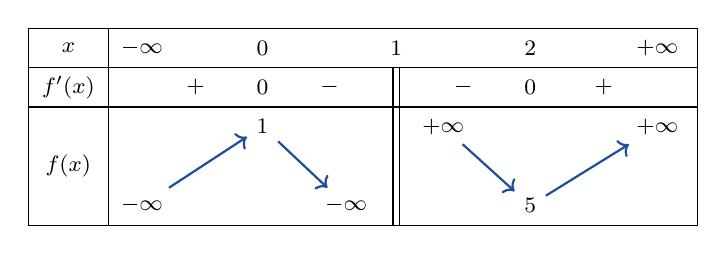
\begin{tikzpicture}[x=0.85cm,y=0.5cm,font=\footnotesize]
\draw (0,0) rectangle (10,-5); \draw (0,-1)--(10,-1); \draw (0,-2)--(10,-2); \draw (1.2,0)--(1.2,-5);
\draw (5.45,-1)--(5.45,-5); \draw (5.55,-1)--(5.55,-5);
\node at (0.6,-0.5){$x$}; \node at (0.6,-1.5){$f^{\prime}(x)$}; \node at (0.6,-3.5){$f(x)$};
\node at (1.7,-0.5){$-\infty$}; \node at (3.5,-0.5){$0$}; \node at (5.5,-0.5){$1$}; \node at (7.5,-0.5){$2$}; \node at (9.4,-0.5){$+\infty$};
\node at (2.5,-1.5){$+$}; \node at (3.5,-1.5){$0$}; \node at (4.5,-1.5){$-$}; \node at (6.5,-1.5){$-$}; \node at (7.5,-1.5){$0$}; \node at (8.6,-1.5){$+$};
\node (m) at (1.7,-4.5){$-\infty$}; \node (a) at (3.5,-2.5){$1$}; \node (b) at (4.75,-4.5){$-\infty$};
\node (c) at (6.2,-2.5){$+\infty$}; \node (d) at (7.5,-4.5){$5$}; \node (p) at (9.4,-2.5){$+\infty$};
\draw[->,cDef,thick] (m)--(a); \draw[->,cDef,thick] (a)--(b); \draw[->,cDef,thick] (c)--(d); \draw[->,cDef,thick] (d)--(p);
\end{tikzpicture}}\end{LTR}\par \par\textbf{(4)} $f(x)-(x+2)=\dfrac1{x-1}$: $(C_f)$ \RR{فوق} المقارب على $]1;+\infty[$ و\RR{تحته} على $]-\infty;1[$.\par\smallskip\begin{LTR}\centering \begin{tikzpicture}[x=0.45cm,y=0.3cm,font=\scriptsize]
\draw[->] (-5,0)--(6,0) node[right]{$x$}; \draw[->] (0,-8)--(0,12) node[above]{$y$};
\draw[cThm,dashed] (1,-8)--(1,12) node[right]{$x=1$};
\draw[cRem,dashed,domain=-5:6] plot (\x,{\x+2}); \node[cRem] at (5.2,9.3){$y=x+2$};
\draw[cDef,thick,domain=-5:0.85,samples=60] plot (\x,{\x+2+1/(\x-1)});
\draw[cDef,thick,domain=1.1:5.6,samples=60] plot (\x,{\x+2+1/(\x-1)}); \node[cDef] at (3.6,8){$C_f$};
\end{tikzpicture}\end{LTR}\par }{50 د}{رسم بالحاسبة للتحقق.}
\Row{}{%
\Lab{cThm!80!black}{حذار}\ نرسم المقاربات أولاً ثم المنحنى.}{}{}
\Row{التقويم}{%
\Lab{cMeth}{تمرين تطبيقي}\par $g(x)=\dfrac{2x+1}{x-1}$.\par\textbf{(1)} بيّن أن $g(x)=2+\dfrac3{x-1}$ واستنتج المقاربات.\par\textbf{(2)} ادرس اتجاه تغير $g$.}{25 د}{تقويم فردي.}
\Row{}{%
\Lab{cEx}{حل التمرين التطبيقي}\par\textbf{(1)} $2+\dfrac3{x-1}=\dfrac{2x-2+3}{x-1}=g(x)$ ؛ \RR{$y=2$} مقارب أفقي و\RR{$x=1$} مقارب عمودي.\par\textbf{(2)} $g^{\prime}(x)=\dfrac{-3}{(x-1)^2}<0$: $g$ \RR{متناقصة تماماً} على كل من $]-\infty;1[$ و $]1;+\infty[$.\par\textbf{واجب منزلي:} مسائل من باب النهايات.\par\smallskip\textbf{ملاحظات حول سير الحصة:} \dotfill}{}{}
\end{Sayr}
\newpage
\ModhHead{21}{3 ت ا}{تحليل}{النهايات ودراسة الدوال}{02 سا}{حل مسائل: دراسة دالة الكلفة المتوسطة}%
{\begin{itemize}\item المشتقات ، النهايات ، المقاربات ، المصطلحات الاقتصادية.\end{itemize}}%
{\begin{itemize}\item دراسة دالة في وضعية اقتصادية وتفسير النتائج.\end{itemize}}%
{المنهاج ، الكتاب المدرسي ، الآلة الحاسبة البيانية. ورق ميليمتري.}
\begin{Sayr}
\Row{مرحلة الانطلاق}{%
\textbf{التهيئة النفسية:} لماذا تكون الكلفة المتوسطة كبيرة جداً لما تكون الكمية المنتجة صغيرة؟}{10 د}{وضعية اقتصادية.}
\Row{التشخيص والاكتشاف}{%
\Lab{cEx}{مسألة}\ الكلفة الإجمالية $C(q)=q^2+10q+400$ (بآلاف الدنانير) ، $q>0$.\par\textbf{(1)} اكتب الكلفة المتوسطة $C_M(q)$.\par\textbf{(2)} احسب نهايتي $C_M$ عند $0^{+}$ و $+\infty$ ، واستنتج المقاربات.\par\textbf{(3)} ادرس اتجاه تغير $C_M$ وعيّن أصغر كلفة متوسطة.\par\textbf{(4)} قارن الكلفة الهامشية والكلفة المتوسطة عند هذه الكمية.}{35 د}{عمل بالأفواج.}
\Row{}{%
\Lab{cDef}{مناقشة النشاط}\par\textbf{(1)} $C_M(q)=\dfrac{C(q)}q=\RR{q+10+\dfrac{400}q}$.\par\textbf{(2)} $\lim\limits_{q\to0^{+}}C_M(q)=\RR{+\infty}$ (الكلفة الثابتة $400$ موزّعة على عدد قليل من الوحدات): محور التراتيب مقارب عمودي. $\lim\limits_{q\to+\infty}C_M(q)=\RR{+\infty}$ و $C_M(q)-(q+10)=\dfrac{400}q\to0$: \RR{$y=q+10$ مقارب مائل} و $C_M$ فوقه.}{}{}
\Row{بناء المعارف}{%
\Lab{cEx}{الدراسة}\par\textbf{(3)} $C_M^{\prime}(q)=1-\dfrac{400}{q^2}=\RR{\dfrac{(q-20)(q+20)}{q^2}}$ ، إشارتها من إشارة $q-20$:\par\smallskip\begin{LTR}\centering \resizebox{0.92\linewidth}{!}{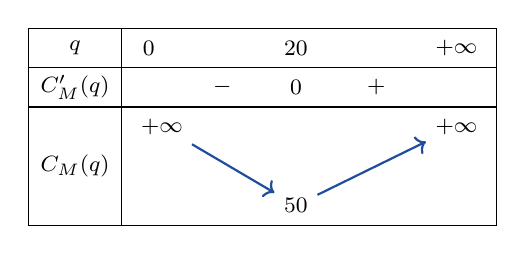
\begin{tikzpicture}[x=0.85cm,y=0.5cm,font=\footnotesize]
\draw (0,0) rectangle (7,-5); \draw (0,-1)--(7,-1); \draw (0,-2)--(7,-2); \draw (1.4,0)--(1.4,-5);
\node at (0.7,-0.5){$q$}; \node at (0.7,-1.5){$C_M^{\prime}(q)$}; \node at (0.7,-3.5){$C_M(q)$};
\node at (1.8,-0.5){$0$}; \node at (4,-0.5){$20$}; \node at (6.4,-0.5){$+\infty$};
\node at (2.9,-1.5){$-$}; \node at (4,-1.5){$0$}; \node at (5.2,-1.5){$+$};
\node (a) at (2,-2.5){$+\infty$}; \node (b) at (4,-4.5){$50$}; \node (c) at (6.4,-2.5){$+\infty$};
\draw[->,cDef,thick] (a)--(b); \draw[->,cDef,thick] (b)--(c);
\end{tikzpicture}}\end{LTR}\par أصغر كلفة متوسطة $C_M(20)=\RR{50}$ ألف دينار.\par\smallskip\begin{LTR}\centering \begin{tikzpicture}[x=0.11cm,y=0.045cm,font=\scriptsize]
\draw[->] (0,0)--(64,0) node[right]{$q$}; \draw[->] (0,0)--(0,125) node[above]{$y$};
\foreach \t in {10,20,30,40,50,60} \draw (\t,1.5)--(\t,-1.5) node[below]{$\t$};
\foreach \t in {25,50,75,100} \draw (1,\t)--(-1,\t) node[left]{$\t$};
\draw[cRem,dashed,domain=0:60] plot (\x,{\x+10}); \node[cRem,right] at (60,70){$y=q+10$};
\draw[cDef,thick,domain=3.7:60,samples=80] plot (\x,{\x+10+400/\x}); \node[cDef] at (8,118){$C_M$};
\draw[cThm,densely dotted] (20,0)--(20,50)--(0,50); \fill[cThm] (20,50) circle (1.2pt);
\end{tikzpicture}\end{LTR}\par \par\textbf{(4)} $C_m(20)=C^{\prime}(20)=2\times20+10=\RR{50}=C_M(20)$.}{50 د}{التفسير الاقتصادي.}
\Row{}{%
\Lab{cRem}{ملاحظات}\ عند أصغر كلفة متوسطة تتساوى الكلفة الهامشية والكلفة المتوسطة.}{}{}
\Row{التقويم}{%
\Lab{cMeth}{تمرين تطبيقي}\par الكلفة الإجمالية $C(q)=2q^2+8q+50$ ، $q>0$.\par\textbf{(1)} اكتب $C_M(q)$ واستنتج مقاربي منحناها.\par\textbf{(2)} عيّن الكمية التي تجعل الكلفة المتوسطة أصغر ما يمكن ، وقارنها بالكلفة الهامشية.}{25 د}{نهاية المحور: فرض أو معالجة بيداغوجية.}
\Row{}{%
\Lab{cEx}{حل التمرين التطبيقي}\par\textbf{(1)} $C_M(q)=\RR{2q+8+\dfrac{50}q}$: المقاربان \RR{$q=0$} و\RR{$y=2q+8$}.\par\textbf{(2)} $C_M^{\prime}(q)=2-\dfrac{50}{q^2}=\dfrac{2(q-5)(q+5)}{q^2}$: الأصغر عند $q=5$: $C_M(5)=10+8+10=\RR{28}$ ؛ و $C_m(5)=4\times5+8=\RR{28}$.\par\textbf{واجب منزلي:} مسائل اقتصادية من باب النهايات.\par\smallskip\textbf{ملاحظات حول سير الحصة:} \dotfill}{}{}
\end{Sayr}
\end{document}
